 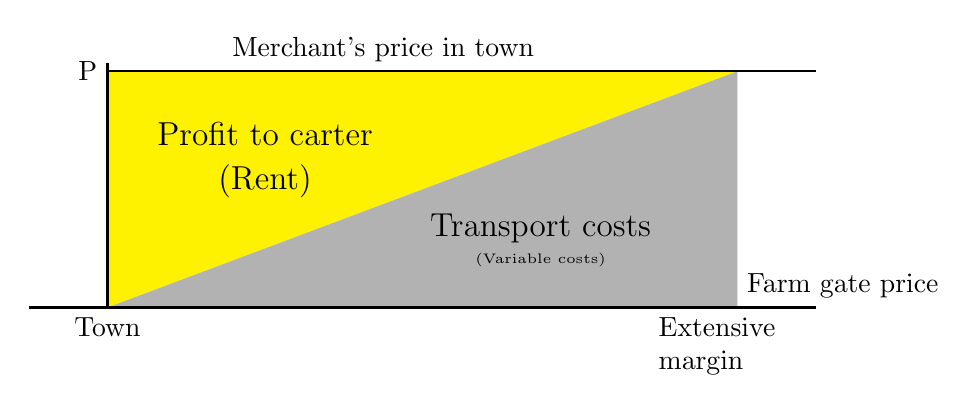
\begin{tikzpicture}[domain=0:2]
%\draw[thick,color=gray,step=.5cm, dashed] (-0.5,-.5) grid (3,3);
%\draw[line width=.01, green ] (0,0) -- (10,0) node[right  ] {Distance};
\node at (1,0) [below] {Town};
\fill[yellow]  (1,0) --(9,3)--(1,3) --cycle;
\fill[gray!60] (9,3) --(1,0)--(9,0) --cycle;

\draw[thick ] (1,3)node[left]{P}  -- (10,3);\node at (4.5,3)[above ] {Merchant's price in town} ;
\draw[thick ] (0,0)  -- (10,0); 

%\draw[thick,color=red] (1.5,0) -- (1.5,1) node[below right] {Fixed cost} -- (1.5,1.5) --(10,3.25)node[above left] {total cost};
\draw[thick] (1,0) -- (1,3.1) ;
\node[below,text width=2cm]at (9,0) {Extensive margin};
%\draw[ultra thick, blue,<-> ] (3,1.8) -- (3,2.5)node[left] {annual rent at a} -- (3,3) ; 
\node at (9,0)[above right] {Farm gate price};
\node  at (6.5,1){\large Transport costs};
\node  at (6.5,.6){\tiny (Variable costs)};
\node  at (3.,2.2){\large Profit to carter};
\node  at (3.,1.6){\large (Rent)};
\end{tikzpicture} 